%% LyX 2.2.2 created this file.  For more info, see http://www.lyx.org/.
%% Do not edit unless you really know what you are doing.
\documentclass[english,a4paper]{article}
\usepackage[T1]{fontenc}
\usepackage[latin9]{inputenc}
\usepackage{geometry}
\geometry{verbose,tmargin=1.5cm,bmargin=1.5cm,lmargin=2cm,rmargin=2cm}
\pagestyle{empty}
\usepackage{float}
\usepackage{amsmath}
\usepackage{graphicx}
\usepackage{wasysym}

\makeatletter

%%%%%%%%%%%%%%%%%%%%%%%%%%%%%% LyX specific LaTeX commands.
%% Because html converters don't know tabularnewline
\providecommand{\tabularnewline}{\\}
\floatstyle{ruled}
\newfloat{algorithm}{tbp}{loa}
\providecommand{\algorithmname}{Algorithm}
\floatname{algorithm}{\protect\algorithmname}

\makeatother

\usepackage{babel}
\usepackage{listings}
\renewcommand{\lstlistingname}{Listing}

\begin{document}

\title{2ID90 International Draught assignment}

\author{Group 19: Daan de Graaf, Yoeri Poels}
\maketitle

\section{Introduction}
In this project we explore the creation of an AI (Artificial Intelligence) to play the game of Draughts, on a 10 $\times$ 10 board configuration, which is that of International draughts. We will create a plugin for the Draughts tournament application provided by the Eindhoven University of Technology, which is used to play / simulate Draughts games. Our plugin/player has to try and find the best possible move in a given timeframe. This is done using a minimax algorithm using alpha-beta pruning, and an evaluation function. In this report we will explain our approach for this, extra optimizations added to try and increase its playing capability, and a review of the outcome. 
\newpage
\section{Alpha-Beta}
We made the decision early on to implement alpha-beta pruning in the single method below, in contrast to having two separate methods that are very similar in an effort to reduce code duplication. We added an extra boolean parameter 'maximize' to indicate whether the algorithm should minimize or maximize the evaluation function. 
We also added a 'depth' parameter to indicate how deep down the tree the algorithm may search. Upon a recursive call the 'maximize' parameter is flipped, and the 'depth' is decreased by 1. If the method is called with depth 0, the heuristic evaluation of the node is returned. 
We have added one more parameter 'didCapture', which is set to true only if the method was called recursively and in the given node state the previous move was a capture. This is only used to make sure that the best move of node is not set to a move that occurs after a capture, as captures do not count towards the depth. 
On top of this we also extend the search depth by two layers if the depth reaches 0 on a node that is not quiet.
The resulting algorithm then becomes:

\begin{algorithm}[H]
\begin{lstlisting}[language=Java,numbers=left,numberstyle={\footnotesize},stepnumber=2,basicstyle={\scriptsize},tabsize=4, mathescape=true]
int AlphaBeta(node, alpha, beta, depth, maximize, didCapture) {
	// Search up to two extra nodes further if the current node is not quiet
	if ((depth <= 0 && isQuiet(node)) || depth <= -2)	 { return Evaluate(node); }
	int bestValue = maximize ? $\infty$ : $-\infty$;
	
	for (move : PossibleMoves(node) {
		node.doMove(move);	// Apply this move so we can evaluate the state
		int newDepth;
		if (move.isCapture()) {
			newDepth = depth; // Do not count captures in the search depth	
		} else {
			newDepth = depth - 1;
		}
	
		int value = AlphaBeta(node, alpha, beta, newDepth, !maximize, m.isCapture());
		if (maximize && value >= bestValue) {
			bestValue = value;
			if (depth == searchDepth && !didCapture) {
				// We are at the root of the search tree
				node.setBestMove(move);				
			}
			
			if (bestValue >= beta) {
				node.undoMove(move); // Undo move for clean return
				return bestValue;
			}
		}
		else if (!maximize && value <= bestValue) {
			bestValue = value;
			if (depth == searchDepth && !didCapture) {
				node.setBestMove(move);			
			}
			
			if (bestValue <= alpha) {
				node.undoMove(move);
				return bestValue;			
			}
		}
		node.undoMove(move); // Undo the move so we can reuse the node for the next iteration of the loop		
	}
	return bestValue;
	
}
\end{lstlisting}

\caption{\label{alg:AlphaBeta}AlphaBeta}
\end{algorithm}


\section{Iterative Deepening}

We implement iterative deepening by first running Algorithm \ref{alg:AlphaBeta} with an initial search depth 'baseSearchDepth' and storing this move. Then while we still have time we keep repeating this process with an increasing search depth until the time runs out. When the time runs out the alphaBeta method throws an AIStoppedException, which is caught here and  The algorithm is given by:

\begin{algorithm}[H]
\begin{lstlisting}[language=Java,numbers=left,numberstyle={\footnotesize},stepnumber=2,basicstyle={\scriptsize},tabsize=4, mathescape=true]
Move IterativeDeepening(State s) {
        bestMove = null;
        try {
            node = new Node(s.clone());
            
            // Set to initial search depth
            searchDepth = baseSearchDepth;
            // Loop while not interrupted
            while (true) {
                bestValue = alphaBeta(node, $-\infty$, $\infty$, searchDepth, s.isWhiteToMove(), false);
                bestMove = node.getBestMove();
                if ((bestValue == MAX_VALUE && s.isWhiteToMove())
                        || (bestValue == MIN_VALUE && !s.isWhiteToMove())) {
                    // We have a winning strategy
                    break;
                }

                searchDepth++; // Increase the search depth for the next iteration
            }

        } catch (AIStoppedException ex) {
        		// Our time is up, return the best move according to the highest search depth reached
	        	return bestMove;
        }
}
\end{lstlisting}

\caption{\label{alg:Iterative}IterativeDeepening}
\end{algorithm}

\newpage
\section{Evaluation}

Our evaluation of board state \emph{s} is split up in several parts, with each having a different weight. The total evaluation-score is based on an evaluation of the \textbf{amount of pieces and kings}, the \textbf{tempi}, \textbf{balance} and \textbf{coherence} of both sides, and the \textbf{mobility}. \\ \\
The score for the amount of pieces/kings \emph{piecesScore} is calculated in the following way:
\begin{equation}
piecesScore(s) = (\fullmoon(s) + 3 \cdot \fullmoon king(s)) - (\newmoon(s) + 3 \cdot \newmoon king(s))
\end{equation}
where for board state \emph{s}, \fullmoon(s) and \newmoon(s) are the number of white and black pieces, and \fullmoon king(s) and \newmoon king(s) are the number of white and black kings, respectively.\\ Kings are given a value of 3 because this is generally accepted to be its value relative to normal pieces$^[1]$. \\ We use $piecesScore$ since having more pieces / the opponent losing pieces means you are more likely to win, since the end goal is the opponent having no pieces left, and having more pieces puts you in a stronger position to take capture their pieces and win. \\ \\
The score for the tempi of both sides \emph{tempiScore} is calculated in the following way: 
\begin{equation}
tempiScore(s) = whiteTempi(s) - blackTempi(s) \\
\end{equation}
where \emph{whiteTempi} and \emph{blackTempi} are the following:\\
\begin{algorithm}[h]
	\begin{lstlisting}[language=Java,numbers=left,numberstyle={\footnotesize},stepnumber=2,basicstyle={\scriptsize},tabsize=4]
	int whiteTempi(State s) {
		whiteTempi = 0;
		for (every white piece in state s) { 
			whiteTempi = whiteTempi + distance from white piece to bottom row (in number of rows);
		}
		return whiteTempi;
	}
	
	int blackTempi(State s) {
		blackTempi = 0;
		for (every black piece in state s) {
			blackTempi = blackTempi + distance from black piece to top row (in number of rows);
		}
		return blackTempi;
	}
	\end{lstlisting}
\end{algorithm} \\
An example of whiteTempi (total value being 23) is shown in Figure \ref{fig:WhiteTempi}: 
\begin{figure}[bh]
	\begin{centering}
		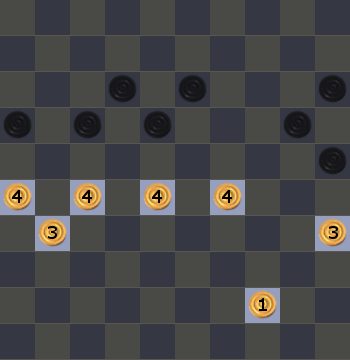
\includegraphics[scale=0.35]{tempi_white.png}
		\par\end{centering}
	\emph{\caption{\label{fig:WhiteTempi}An example of whiteTempi}
	}
\end{figure}

We use this to give extra value to pieces closer to the other side, because it's more likely to become a king when it's closer. \\ \\
The score for balance, \emph{balanceScore}, is calculated in the following way: \\ \\
\begin{equation}
balanceScore(s) = blackUnbalance(s) - whiteUnbalance(s)
\end{equation}
Where blackUnbalance(s) and whiteUnbalance(s) are the amount of pieces it has more on one side, than on the other side: $|$amount of pieces in two leftmost columns $-$ amount pieces in two rightmost columns$|$ (amount of pieces being only black pieces in blackUnbalance(s), and white in whiteUnbalance(s), respectively). An example of this is in figure \ref{fig:Balance}.
\begin{figure}[!h]
	\begin{centering}
		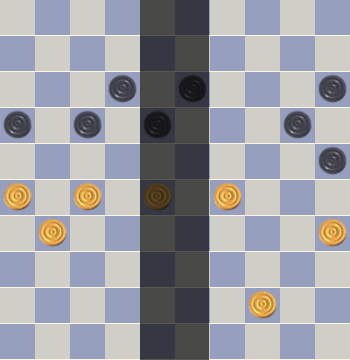
\includegraphics[scale=0.35]{balance_both.png}
		\par\end{centering}
	\emph{\caption{\label{fig:Balance}Balance evaluation}
	}
\end{figure}
As seen in this figure, on the left side of the board there are 3 white pieces, on the right side there are also 3 white pieces. This makes the \emph{whiteUnbalance(s)} = $|3-3|=0$ (blackUnbalance(s) has the exact same score / calculation in this figure). \\
We use this because it values having a balanced state on your side, which should protect against breakthroughs from the other side $^[1]$, which leads to that side getting a king. \\ \\
The score of the coherence of a side, $coherenceScore$, is calculated based on the neighbours of all pieces. Every piece gets a point for a neighbour, and also gets points for being at an edge of the board (since this functions similarly to having a neighbour there). The total calculation is then simply the following:
\begin{equation}
coherenceScore(s) = whiteCoherence(s) - blackCoherence(s)
\end{equation}
whiteCoherence and blackCoherence are then calculated the following way: \\
\begin{algorithm}[!h]
	\begin{lstlisting}[language=Java,numbers=left,numberstyle={\footnotesize},stepnumber=2,basicstyle={\scriptsize},tabsize=4]
	int whiteCoherence(State s) {
		whiteCoherence = 0;
		for (every white piece in state s) {
			whiteCoherence = whiteCoherence + amount of white pieces/sides surrounding this piece;
		}
		return whiteCoherence;
	}
	
	int blackCoherence(State s) {
		blackCoherence = 0;
		for (every black piece in state s) {
			blackCoherence = blackCoherence + amount of black pieces/sides surrounding this piece;
		}
		return blackCoherence;
	}
	\end{lstlisting}
\end{algorithm}
\\An example of blackCoherence is shown in Figure \ref{fig:BlackCoherence}, (resulting in blackCoherence(s) = 16). 
\begin{figure}[!h]
	\begin{centering}
		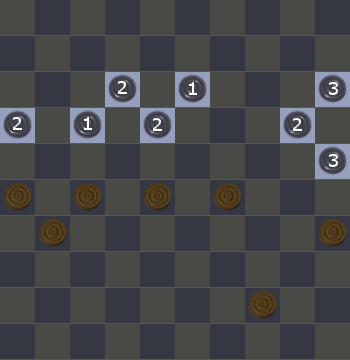
\includegraphics[scale=0.35]{coherence_black.png}
		\par\end{centering}
	\emph{\caption{\label{fig:BlackCoherence}An example of blackCoherence}
	}
\end{figure}
\\ We use coherenceScore since it gives an idea of how well pieces are grouped together, and how well they are protected: Since a piece cannot be captured if it has a 'neighbouring' piece in the direction of the (attempted) capture, having a high coherenceScore makes the pieces 'safer'. \\ \\
The \emph{mobilityScore} is simply the amount of possible moves in that state. We use this to evaluate since having a higher mobility, more moves available, means there are still more options open, more control over the game for the player, which can aid in winning the game. \\ \\
All these different scores will have to be combined into one final score to evaluate a state, using different weights for the scores. The final score will then be: \\
$score(s) = w_{1} \cdot piecesScore(s) + w_{2} \cdot tempiScore(s) + w_{3} \cdot balanceScore(s) + w_{4} \cdot coherenceScore(s) + w_{5} \cdot mobilityScore(s)$. \\
To figure out if all pieces of the evaluation function worked properly they were enabled one by one (given a weight $\neq 0$) and tested against a previous version. Every time a new function was enabled it beat the old version. We ended up with the following weights: $w_{1} = 80, w_{2} = 4, w_{3} = 4, w_{4} = 4, w_{5} = 1$. However these weights were still rough guesses so machine learning was used to find better weights. \\
In every generation of our machine learning algorithm all 'versions' of the draughts player were matched with another one, to create a match. The winners of the matches were then crossed over and mutated for the next generation. This was done for roughly 80 generations of 50 elements. At the end these players played a 'death match' versus eachother, a knockout bracket to determine the strongest player. We then also tested this player against the player we made ourselves, and it beat our old player aswell. So we went with the outcome of the machine learning as our final player. The score evaluation for this, and our final player is: \\
$score(s) = 60 \cdot piecesScore(s) + 6 \cdot tempiScore(s) + 11 \cdot balanceScore(s) + 1 \cdot coherenceScore(s) + 3 \cdot mobilityScore(s)$.

\section{Custom extensions}
We have handled quiescence in Algorithm \ref{alg:AlphaBeta}, where at depth 0 we also check if the board state is currently quiet. If it is we return the heuristic evaluation of the node, otherwise we allow the search to continue op to 2 levels further in the tree. To check if a state is quiet we use the following simple algorithm:
\begin{algorithm}[h]
\begin{lstlisting}[language=Java,numbers=left,numberstyle={\footnotesize},stepnumber=2,basicstyle={\scriptsize},tabsize=4, mathescape=true]
Move IsQuiet(State s) {
        moves = s.getMoves();
        if (moves.isEmpty()) {
        		// No pieces are left on the board
        		return true;
        	}
        return !moves.get(0).isCapture();
}
\end{lstlisting}

\caption{\label{alg:Iterative}IsQuiet}
\end{algorithm}

We also ignore obliged moves in the search depth, as can be seen on line 9-10 of Algorithm. \ref{alg:AlphaBeta}.

These extensions did make the AI stronger, but only slightly. When an otherwise identical version without these modifications (A) plays against the version with these extensions (B), A will draw B when A is white. But when B is white, it will win by a slight edge it has with the extensions. This is most visible in the end game:

\begin{figure}[H]
	\begin{centering}
		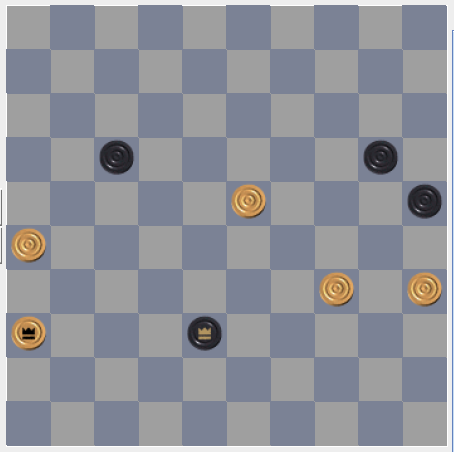
\includegraphics[scale=0.35]{extensions1.png}
		\par\end{centering}
	\emph{\caption{The game is nearly tied in piece count and the two kings suggest a draw outcome}
	}
\end{figure}

\begin{figure}[H]
	\begin{centering}
		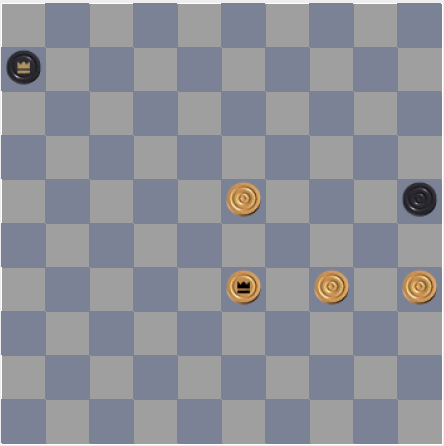
\includegraphics[scale=0.35]{extensions2.png}
		\par\end{centering}
	\emph{\caption{A is to move and has to strike the king and another piece, allowing B to capture the king and force A to put its last piece in harms way.}
	}
\end{figure}

\begin{figure}[H]
	\begin{centering}
		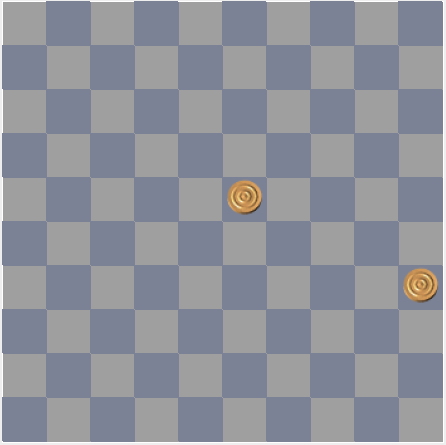
\includegraphics[scale=0.35]{extensions.png}
		\par\end{centering}
	\emph{\caption{B wins by exploring further}
	}
\end{figure}



\section{Results and Conclusions}

The resulting evaluation function (with weights determined by machine learning) as mentioned in section 4 is the following: \\ $score(s) = 60 \cdot piecesScore(s) + 6 \cdot tempiScore(s) + 11 \cdot balanceScore(s) + 1 \cdot coherenceScore(s) + 3 \cdot mobilityScore(s)$. This evaluation function was used as an evaluation for our implementation of minimax with Alpha-beta pruning, using iterative deepening and checking for quiet moves and ignoring obliged moves in the search depth, as extensions. The resulting player was quite strong, neither of us could come close to beating the player, but we are also not Draughts experts. The big test was the draughts tournament. The player ended up going 4-3 (wins-losses) in our pool, leaving us in 3rd place. We think the biggest weaknesses of our player was its lack of checking for certain patterns, possibly not being efficient enough (so other players could search deeper in the tree to find a better move), and the fact that it only played against variations of our player in the machine learning process, leading to overfitting$^{[2]}$ of the parameters.

\section{Contributions}

\begin{tabular}{|c|c|c|c|}
\cline{2-4} 
\multicolumn{1}{c|}{} & \textbf{implementation} & \textbf{documentation} & \textbf{total \#hours}\tabularnewline
\hline 
Daan de Graaf & 60\% & 40\% & 28\tabularnewline
\hline 
Yoeri Poels & 40\% & 60\% & 26\tabularnewline
\hline 
\end{tabular}
\bibliographystyle{plain}

\newpage

\section*{References}
[1] Wieger Wesselink (2017). Computer draughts evaluation. Eindhoven University of Technology.
\\{}[2] Martha K. Smith (2014-06-13). "Overfitting". University of Texas at Austin.
\end{document}
